\documentclass[11pt]{article}
\usepackage[T1]{fontenc}
\usepackage[utf8]{inputenc}
\usepackage[a4paper,margin=1in]{geometry}
\usepackage{graphicx}
\usepackage{booktabs}
\usepackage{amsmath,amssymb}
\usepackage{hyperref}
\usepackage{subcaption}
\usepackage{float}
\usepackage[expansion=false]{microtype}
\usepackage{enumitem}
\usepackage{xcolor}
\usepackage{siunitx}
\usepackage{array}
\setlength{\emergencystretch}{3em}
\hypersetup{colorlinks=true,linkcolor=black,citecolor=black,urlcolor=blue}
\sisetup{round-mode=places,round-precision=3}

\title{Degree-Preserving Structural Perturbations and CDCL Behavior in Tseitin Formulas}
\author{Amandine Morin}
\date{Created 4 October 2026, 13:26:20 CEST (UTC+02:00)}

\begin{document}
\maketitle

\begin{abstract}
Tseitin formulas provide a controlled setting in which graph structure can be related to propositional proof search. We study randomized degree-preserving double-edge swaps of a 4-regular ring on 80 vertices, holding the 160 edges and complete degree sequence fixed. In a 300-instance discovery campaign with instrumented Kissat~4.0.4, the fraction exceeding a 60-second budget rises from 3.3\% at 16 requested swaps to 36.7\% at 20, 76.7\% at 24, 96.7\% at 32, and 100\% at 48 and 80. A separate 200-instance confirmation replicated the prespecified within-swap associations: runs censored under the campaign presentation had higher global efficiency and lower modularity at both 20 and 24 swaps.

Exploratory censored accelerated-failure-time (AFT) analyses yielded positive predictive gains for global efficiency in several evaluations beyond the stated approximate baselines. After a fixed-graph pilot, we prespecified a robustness campaign with 60 outcome-blind selected graphs and five joint variable-renumbering and clause-order presentations each. In this sample, 24 of 60 graphs exhibited both resolved and censored outcomes across the five presentations. Higher efficiency retained a negative adjusted association with resolution probability (coefficient $-1.525$, graph-bootstrap 95\% interval $[-2.446,-0.688]$), including after a treewidth-squared sensitivity, but its held-out log-score gain was $+0.02265$ with interval $[-0.01130,+0.05959]$. Under the frozen three-part rule, robustness was not established: the adjusted association was recovered, whereas additional predictive value was inconclusive. This does not imply absence of an effect.
\end{abstract}

\section{Introduction}

Tseitin contradictions connect a graph to an unsatisfiable system of parity constraints and have long served as canonical objects in proof complexity~\cite{Tseitin1970,BenSassonWigderson2001}. Their theoretical study establishes strong links among expansion, width, treewidth, and Resolution proof size~\cite{AlekhnovichRazborov2011,ItsyksonEtAl2022,deColnetMengel2023}. Modern conflict-driven clause-learning (CDCL) solvers can be viewed through the same proof-system lens, but practical proof search depends on interacting heuristics whose behavior is not determined by proof size alone. Carefully structured theoretical benchmarks are therefore useful for studying how solver behavior changes under controlled modifications~\cite{ElffersEtAl2018}.

We ask how a controlled structural perturbation of a graph translates into the behavior of a modern CDCL solver on the corresponding Tseitin formula. Starting from a 4-regular ring, we apply a prescribed number of randomized degree-preserving double-edge swaps. This design keeps $n$, $|E|$, every vertex degree, and hence the entire degree sequence fixed. At the same time, multiple structural properties change together, so the construction does not isolate a single causal topological variable.

The discovery campaign contains 30 seeds at each of ten perturbation levels, for 300 deterministic instances. The fraction of runs reaching the 60-second limit rises from 3.3\% at 16 requested swaps to 36.7\% at 20, 76.7\% at 24, and 96.7\% at 32. The strongest observed increase occurs through 16, 20, and 24 swaps. We use \emph{empirical transition} only as shorthand for this rapid increase in the probability of exceeding the fixed budget. A continuous increase in times can produce the same pattern as more of the distribution crosses 60 seconds; with one graph size, one degree, and one budget, we do not identify an intrinsic transition, critical point, or growth law.

The discovery analysis identified direction-consistent within-swap associations at 20 and 24 swaps. We then froze a targeted independent-confirmation protocol before execution and generated 100 new instances at each level using disjoint seed ranges. The 200 confirmation runs were analyzed separately from the discovery campaign; no confirmatory test pools the two samples.

After confirmation, we conducted a censored AFT analysis and a fixed-graph presentation-sensitivity pilot. The pilot motivated a separate 300-run robustness campaign whose graph selection, presentation distribution, grouped analysis, cross-validation folds, and decision rule were frozen before execution. We subsequently performed one exploratory effective-dose sensitivity on the number of final edges absent from the seed-matched ring.

Together, the campaigns form a controlled empirical study of one solver on degree-preserving perturbations of a ring, with an independently replicated analysis and explicit presentation controls. They associate perturbation with a rapid change in the probability of exceeding the budget and with systematic solver-trajectory signatures. The normalized-Laplacian spectral gap $\lambda_2$ is one descriptor among clustering, path length, modularity, approximate conductance, and approximate treewidth. The contribution is the controlled design and its bounded empirical evidence, not the discovery of a general structure--difficulty link or of solver sensitivity.

\paragraph{Contributions.}
\begin{itemize}[leftmargin=1.5em]
    \item We conduct a controlled 300-instance study of exact degree-preserving double-edge perturbations of a 4-regular ring, relating fixed-budget outcomes to six graph descriptors and solver-trajectory measurements under one encoding and solver.
    \item In an independent 200-instance campaign whose protocol and decision rules were frozen before execution, we replicate the prespecified within-swap associations of higher global efficiency and lower modularity with censoring.
    \item We measure presentation sensitivity in a fixed-graph pilot and a prespecified 60-graph repeated-presentation campaign, keeping graph-level dependence explicit.
    \item We distinguish the recovered adjusted efficiency association from its inconclusive additional held-out predictive value; complementary AFT and effective-dose analyses remain exploratory.
\end{itemize}

\section{Background and Related Work}

\subsection{Tseitin formulas and proof complexity}

For an undirected graph $G=(V,E)$, associate one Boolean variable with each edge. A charge assignment $c:V\to\{0,1\}$ imposes at every vertex the parity constraint that incident edge variables sum to $c(v)$ modulo two. If $G$ is connected and the total charge is odd, the conjunction is inconsistent. Tseitin formulas were introduced as hard examples for propositional proof systems~\cite{Tseitin1970}.

Resolution width and size are related by the size--width method of Ben-Sasson and Wigderson, with graph expansion providing width lower bounds for Tseitin contradictions~\cite{BenSassonWigderson2001}. Branch-width and automatability have also been studied directly for Tseitin formulas~\cite{AlekhnovichRazborov2011}. More recent results characterize regular Resolution complexity in terms of treewidth: Itsykson, Riazanov, and Smirnov prove tight lower bounds for connected graphs~\cite{ItsyksonEtAl2022}, while de Colnet and Mengel characterize bounded-degree families with short regular Resolution refutations~\cite{deColnetMengel2023}. Thus, the general connection from graph structure to Tseitin proof complexity is established prior work, not a novelty claim of this paper. For their specific 3-CNF family of two contradictory chained parity encodings on $n$ input variables---one ordered identically and the other obtained by a negation-preserving literal bijection with one sign flip---Chew and Heule documented empirical CDCL difficulty and constructed $O(n\log n)$-line DRAT refutations without additional variables by reusing the encoding's Tseitin variables~\cite{ChewHeule2020}. Chew et al. later identified randomized reordered encodings as Tseitin formulas, proved linear treewidth with high probability and corresponding exponential Resolution hardness, and reported empirical CDCL runtime increasing with treewidth~\cite{ChewEtAl2024}. Their construction varies order within parity encodings; ours perturbs the underlying graph while preserving every degree and keeps within-clause literal order fixed.

The campaign's chained-XOR CNF is, clause for clause, the canonical Tseitin formula $T(H,q')$ on the connected subcubic gadget graph $H$ obtained by expanding each degree-four vertex (Appendix~\ref{app:gadget}). Consequently, the known regular-Resolution bounds apply to this representation with $\operatorname{tw}(H)$ as the relevant parameter~\cite{ItsyksonEtAl2022,deColnetMengel2023}. In stronger and distinct systems, Buss and Thapen construct polynomial-size refutations of canonical Tseitin contradictions in $\mathrm{SPR}^{-}$; their polynomial simulations separately yield polynomial-size $\mathrm{DRAT}^{-}$ and Extended Resolution refutations~\cite{BussThapen2021}. These proof-existence results concern systems distinct from the actual Kissat search process: they neither imply that its operations and heuristics efficiently discover those constructions nor determine observed search time.

\subsection{Ring perturbations, small-world structure, and SAT}

The classical Watts--Strogatz construction begins with a ring lattice and probabilistically rewires edges, producing a conceptual interpolation between ordered and disordered networks~\cite{WattsStrogatz1998}. Roli studied the effect of small-world structure on local search for SAT~\cite{Roli2005}. Our construction is a methodological neighbor, not the same graph model: standard Watts--Strogatz rewiring need not preserve every vertex degree, whereas our double-edge swaps preserve all degrees exactly.

Structural SAT research has connected community structure and modularity to industrial instances and learned clauses~\cite{AnsoteguiEtAl2012,AnsoteguiEtAl2019}. Ansótegui et al. also used community structure to identify relevant learned clauses~\cite{AnsoteguiEtAl2015}. These results motivate measuring modularity and clause behavior, but the present graph-level modularity is computed on the original Tseitin graph, not on a variable--clause graph, and should not be conflated with those representations.

Singh et al. formalize proofdoors as sequences of interpolants between formula chunks and connect small proofdoors to short Resolution refutations and polynomial-time refutations by specified CDCL configurations~\cite{SinghEtAl2026}. In a distinct BMC setting, Zhang et al. report that scrambling CNF presentation degrades solver performance and yields larger proofdoors, motivating explicit controls for presentation~\cite{ZhangEtAl2026}. Their BMC families, representation, and scaling response differ from our within-stratum Tseitin fixed-budget associations, so neither result refutes the other and our modularity measurements are not a universal predictor. Our instrumentation does not construct or measure proofdoors.

\subsection{Runtime variability, randomization, and presentation}

Runtime variability in complete SAT search is established prior work. Gomes, Selman, and Kautz introduced controlled randomization of branching choices---random tie-breaking, widened by a heuristic-equivalence window when exact ties are rare---together with cutoff-based restarts~\cite{GomesEtAl1998}. They used variable numbering as an illustrative example of a seemingly irrelevant detail that can change runtime, but did not report a controlled experiment with uniform identifier bijections. Later experiments characterized heavy-tailed cost distributions for randomized backtracking on selected SAT and CSP instances and evaluated rapid randomized restarts, while cautioning that this behavior was not universal~\cite{GomesEtAl2000}. The second-edition \emph{Handbook of Satisfiability} chapter reviews how variable and value selection, including tie-breaking, can produce extreme runtime variation and how randomization and restarts can exploit it~\cite{GomesSabharwal2021}. These concepts are related but not interchangeable. Solver randomization changes internal choices; presentation transformations rename variables or reorder clauses while leaving semantics unchanged; a heavy-tail claim concerns a runtime distribution; a restart policy deliberately interrupts and relaunches search; and wall-clock variation can additionally reflect the execution environment. Our pilot and repeated-presentation campaign show changes of status under a fixed 60-second budget. They neither establish a heavy-tailed runtime distribution nor test the effectiveness of restarts.

\subsection{CDCL diagnostics and stronger parity reasoning}

Literal block distance (LBD) was proposed as a learned-clause quality measure and underlies the Glucose line of solvers~\cite{AudemardSimon2009}. We use a Kissat glue-bin proxy rather than exact per-clause LBD, and we separately report usage, unused fraction, and lifetime for the instrumented subset of large redundant learned clauses.

Theoretical benchmarks can reveal where practical CDCL proof search succeeds or fails despite known proof-system properties~\cite{ElffersEtAl2018}. Recent systems also illustrate that Tseitin and parity instances can behave differently under stronger representations. Extended Resolution Clause Learning introduces extension variables at dual implication points and is implemented in xMapleLCM~\cite{BussEtAl2026}. CDCL$(\oplus)$ and its Xorcle implementation reason with disjunctions of parity equations~\cite{BeameSun2026}. We did not test either system; they motivate comparisons beyond standard CDCL in future work.

\section{Experimental Method}

\subsection{Degree-preserving ring perturbation}

We fix $n=80$ and degree $d=4$. The base graph is the undirected regular ring in which each vertex is connected to the two nearest vertices on either side. It has
\[
|E|=\frac{nd}{2}=160.
\]
For each seed, vertex labels are first permuted using \texttt{std::mt19937}. The generator then performs randomized double-edge swaps. Given two current edges $(a,b)$ and $(c,d)$ with four distinct endpoints, it chooses one of the pairings $(a,c),(b,d)$ or $(a,d),(b,c)$. A proposal is rejected if it selects the same edge twice, shares an endpoint, creates a self-loop, creates duplicate proposed edges, or creates an edge already present after temporary removal of the selected pair. Rejected proposals restore the original pair and do not count.

The scheme was historically inspired by Watts--Strogatz in that it starts from a ring and progressively disrupts local structure. However, it is not standard Watts--Strogatz rewiring. It preserves $n$, $|E|$, every degree, and the complete degree sequence. The first relevant implementation parameter is therefore called the \emph{historical rewiring parameter $p$}; it is not a per-edge probability. It requests
\[
S(p)=\operatorname{round}\bigl(p\,10|E|\bigr)
\]
successful double-edge swaps. Table~\ref{tab:mapping} gives the complete mapping. Multiple swaps can touch or reverse previously modified edges, so $S(p)$ is not the number of final edges differing from the base ring.

\begin{table}[t]
\centering
\caption{Historical parameter and requested successful double-edge swaps.}
\label{tab:mapping}
\begin{tabular}{rrrrrrrrrrr}
\toprule
$p$ & .0000 & .0025 & .0050 & .0075 & .0100 & .0125 & .0150 & .0200 & .0300 & .0500\\
\midrule
$S(p)$ & 0 & 4 & 8 & 12 & 16 & 20 & 24 & 32 & 48 & 80\\
\bottomrule
\end{tabular}
\end{table}

All requested swaps succeeded in the campaign. The implementation would fail rather than silently return fewer swaps. The median number of final edges absent from the seed-matched unperturbed ring was, respectively, $0,8,16,23,30,36,42,54,73,$ and $99.5$; these values confirm why swap count and final edge difference must be distinguished.

\subsection{Tseitin encoding and reproducibility}

We use seeds $0,\ldots,29$ at each perturbation level. After graph generation, the same pseudorandom stream generates independent Bernoulli$(1/2)$ vertex charges. If their parity is even, the charge at vertex~0 is flipped, ensuring odd total charge and an unsatisfiable connected Tseitin instance. Each degree-4 parity constraint is encoded as a chain of three binary XOR gates, each gate using the standard four-clause CNF encoding, followed by a unit clause fixing the final parity. Every instance has 400 variables and 1,040 clauses.

The graph and CNF are deterministic for $(n,d,p,\text{seed})$. Every instance has a unique identifier, an exported edge list, and a 64-bit FNV-1a CNF hash. Repeated generation in the campaign smoke test produced identical hashes, and all stored hashes were validated before completed runs were accepted during resume.

\subsection{Solver protocol and censoring}

We run Kissat~4.0.4 with a 60-second limit, sequentially with one solver process at a time. The campaign contains $10\times30=300$ instances. A completed refutation has status \texttt{UNSAT}; a run reaching the limit has status \texttt{UNKNOWN} and is treated as right-censored. The observed wall-clock duration of a censored run records exposure to the limit, not an exact solving time. Consequently, timeout fractions use all runs, while runtime summaries and Figure~\ref{fig:runtime} use resolved runs only. We do not replace censored observations by 60 seconds in runtime correlations.

For every run we record conflicts, decisions, propagations, propagations per conflict, and an approximate mean LBD. The latter is a weighted mean derived from Kissat glue-usage bins; a ranged bin is represented by its midpoint. It is therefore consistently labeled an approximate Kissat glue proxy. Timeout runs can contribute solver metrics accumulated over their observed 60-second trajectories, but these are not completed-refutation measurements.

The local instrumentation additionally tracks large redundant learned clauses stored in the clause arena. Within that scope, it records propagation and conflict-analysis uses, the unused fraction, and lifetime in conflicts. These values are exact within the tracked scope but do not cover the full learned-clause database.

\paragraph{Executable, environment, checks, and artifacts.}
The campaigns used an instrumented Kissat executable reporting version~4.0.4; reported times therefore apply to this instrumented build rather than to an unmodified distribution binary. The verified SHA-256 values were:
\begin{itemize}[nosep,leftmargin=1.5em]
    \item instrumented Kissat: \texttt{11b45a2307295965e9966b5bb779f781}\\
    \texttt{c42df9af0b82717d6796ecac80d3fab6};
    \item local runner: \texttt{15d2ab13c8a52802b15a492e80a32edb}\\
    \texttt{7fec9d6bedc1c97cda1b27ec344b0cd7}.
\end{itemize}
The invocation was \texttt{timeout --preserve-status -k 1s 60s}\allowbreak\texttt{ <instrumented-kissat> --time=60 <cnf>}, with no additional solver option, and runs were sequential. Thus both an external 60-second wall-clock limit and Kissat's internal 60-second time limit were active. The archived logs do not establish which mechanism ended each censored run. Archived confirmation metadata report Python~3.12.3, NetworkX~2.8.8, and NumPy~1.26.4; the AFT environment additionally records SciPy~1.11.4 and Linux~6.6.87.2 under WSL2 with glibc~2.39. Processor model, physical core allocation, RAM, storage, host load, and host-operating-system details were not recorded.

Connectivity was checked on every exported discovery graph with \texttt{networkx.is\_connected}; confirmation validation required 160 distinct loop-free edges, degree four at every vertex, and \texttt{networkx.is\_connected}. The AFT audit rechecked all 300 discovery and 200 confirmation graph hashes and reproduced the stored structural quantities. Archived experiment artifacts are retained locally under \nolinkurl{experiments/}. They include campaign protocols and reports, graph and CNF sources, manifests and metadata, result tables, analysis scripts, and recorded checks for the discovery, confirmation, AFT, presentation-pilot, repeated-presentation, and effective-dose analyses. These local files are not presented as an anonymized reviewer-accessible supplement, and no public availability is claimed.

\subsection{Structural metrics}

All graph metrics are computed once on the original graph used to construct the formula, never on the CNF variable--clause graph. We measure: (i) the second eigenvalue $\lambda_2$ of the normalized Laplacian; (ii) average clustering coefficient; (iii) average shortest-path length; (iv) modularity of the partition returned by NetworkX greedy modularity communities; (v) an approximate conductance, defined as the minimum conductance among nontrivial communities proposed by that partition; and (vi) approximate treewidth returned by NetworkX \texttt{treewidth\_min\_fill\_in}. The last two values are approximations, not exact optima.

\subsection{Prespecified independent confirmation}

The independent confirmation used a protocol frozen before execution; it was not a public preregistration. It retained $n=80$, $d=4$, the historical degree-preserving ring generator, the Tseitin encoding, Kissat~4.0.4, all solver options, and the 60-second censoring rule. It targeted only 20 requested successful swaps ($p=.0125$) and 24 requested successful swaps ($p=.0150$), with 100 new valid instances at each level. The disjoint seed ranges were 1000--1099 at 20 swaps and 2000--2099 at 24 swaps.

Runs were sequential and alternated deterministically: for each index, the 20-swap instance was followed by the corresponding 24-swap instance. The same pseudorandom stream continued from graph generation to charge generation, and the generator was required to complete exactly the requested number of successful swaps. As in the discovery campaign, requested swaps are not the number of final changed edges because later swaps can revisit or reverse earlier changes. Accumulated results were saved after every run with validated identifiers, paths, and CNF hashes for safe resume.

Only two graph metrics were confirmatory. Global efficiency was the NetworkX mean reciprocal shortest-path distance, and modularity used the single partition returned by NetworkX greedy modularity communities. Average shortest-path length is highly redundant with global efficiency and was not counted as an independent confirmatory hypothesis. Within each swap level, censored and resolved groups were compared by the existing two-sided asymptotic Mann--Whitney implementation. Cliff's delta is defined as censored minus resolved and was assigned a deterministic 2,000-resample percentile-bootstrap 95\% interval.

The primary hypothesis required positive Cliff's delta and raw $p<.05$ for global efficiency at both levels. The secondary hypothesis required negative delta and Holm-adjusted $p<.05$ for modularity at both levels, with Holm correction across exactly the two modularity tests. Discovery and confirmation data were not pooled for these decisions.

\subsection{Prespecified repeated-presentation robustness protocol}

Before running the larger presentation campaign, we excluded the eight pilot graphs and selected 30 graphs without replacement at each confirmation level using deterministic shuffles that received only instance identity, swap level, generation seed, and frozen plan index. Status, runtime, and structural metrics were unavailable to the selection function. The post-exclusion source population contained 96 graphs per level.

Each selected source CNF received five new presentations. Every presentation combined an independent uniform bijection of all 400 variable identifiers with an independent uniform permutation of all 1,040 clauses; charges, literal signs, and within-clause literal order were fixed. The 300 sequential Kissat runs retained the same options and 60-second budget. The analysis unit was the graph, with response equal to the number of resolutions before 60 seconds out of five. The baseline logistic model contained swap stratum and min-fill treewidth; the extension added global efficiency.

Uncertainty for coefficients used a 5,000-resample bootstrap of whole graphs within swap level, refitting each model while retaining full-sample scaling. Five-fold prediction kept all presentations of a graph together, balanced graphs within level, and learned standardization only from training graphs. The binary log score for $y$ resolutions and probability $q$ was $\{y\log q+(5-y)\log(1-q)\}/5$. Its gain interval resampled graph-level out-of-fold score differences while holding predictions fixed, so it is conditional and excludes full retraining variability. Robustness required (i) a negative adjusted efficiency coefficient with a 95\% interval excluding zero, (ii) a positive held-out score gain with an interval excluding zero, and (iii) no direction reversal after adding squared standardized treewidth to both models.

\section{Results}

\subsection{Rapid increase in the probability of exceeding 60 seconds}

All 300 runs completed without execution errors: 176 were resolved as \texttt{UNSAT}, and 124 reached the limit. Figure~\ref{fig:timeouts} and Table~\ref{tab:main} show the central empirical result. No run timed out through 12 requested swaps. The timeout fraction then rises from 1/30 at 16 swaps to 11/30 at 20, 23/30 at 24, and 29/30 at 32. Every run timed out at 48 and 80 swaps. The probability of exceeding the fixed budget increases most rapidly through 16, 20, and 24 swaps. This binary censoring pattern does not distinguish an intrinsic transition from continuously growing times crossing the budget.

\begin{figure}[t]
\centering
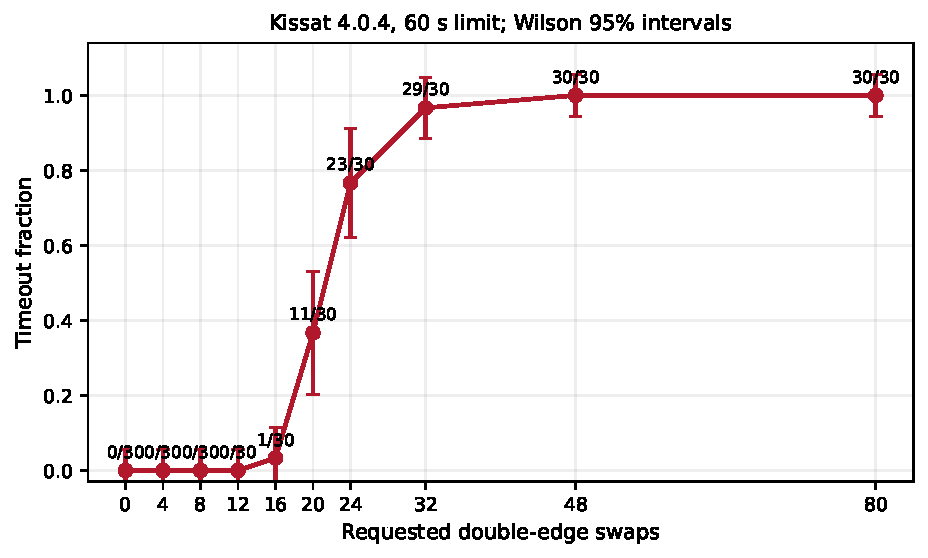
\includegraphics[width=.78\linewidth]{figures_20261003/timeout_fraction_vs_requested_swaps.pdf}
\caption{Fraction of runs reaching the 60-second limit versus requested double-edge swaps. Labels give censored runs out of 30; bars are Wilson 95\% binomial intervals. The historical parameter values are listed in Table~\ref{tab:main}.}
\label{fig:timeouts}
\end{figure}

\begin{table}[H]
\centering
\small
\caption{Main results. Runtime statistics contain resolved runs only; ``--'' means no run resolved. Timeout observations are right-censored.}
\label{tab:main}
\begin{tabular}{rrrrrrcc}
\toprule
$p$ & swaps & $N$ & UNSAT & censored & timeout frac. & resolved median (s) & resolved IQR (s)\\
\midrule
.0000 & 0  & 30 & 30 & 0  & 0.000 & 0.015 & [0.013, 0.021]\\
.0025 & 4  & 30 & 30 & 0  & 0.000 & 0.025 & [0.022, 0.028]\\
.0050 & 8  & 30 & 30 & 0  & 0.000 & 0.066 & [0.038, 0.103]\\
.0075 & 12 & 30 & 30 & 0  & 0.000 & 0.277 & [0.131, 0.457]\\
.0100 & 16 & 30 & 29 & 1  & 0.033 & 1.783 & [0.466, 7.599]\\
.0125 & 20 & 30 & 19 & 11 & 0.367 & 7.193 & [1.778, 18.302]\\
.0150 & 24 & 30 & 7  & 23 & 0.767 & 11.579 & [5.988, 23.917]\\
.0200 & 32 & 30 & 1  & 29 & 0.967 & 29.488 & [29.488, 29.488]\\
.0300 & 48 & 30 & 0  & 30 & 1.000 & -- & --\\
.0500 & 80 & 30 & 0  & 30 & 1.000 & -- & --\\
\bottomrule
\end{tabular}
\end{table}

\subsection{Runtime growth among resolved instances}

Figure~\ref{fig:runtime} shows only completed refutations. Their median runtime grows from 0.015 seconds at zero swaps to 1.783 seconds at 16, 7.193 seconds at 20, and 11.579 seconds at 24. At 32 swaps only one instance resolved, in 29.488 seconds, so that point is not a distributional estimate. No runtime median exists at 48 or 80 swaps. The figure deliberately does not plot censored runs at 60 seconds as if they had resolved there.

These conditional medians describe only the progressively selected subset resolving within the budget. They are not unbiased estimates of unconditional performance and cannot identify a growth law.

\begin{figure}[t]
\centering
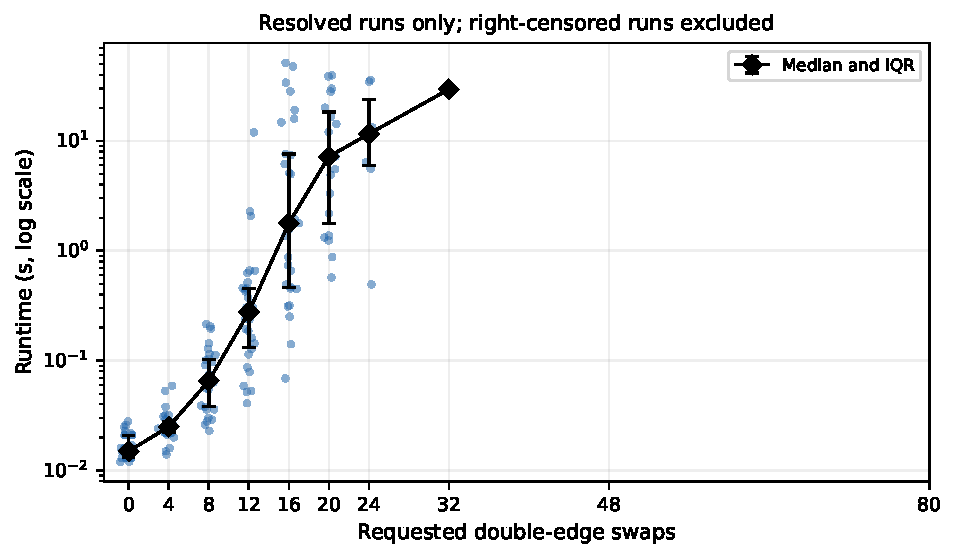
\includegraphics[width=.78\linewidth]{figures_20261003/resolved_runtime_vs_requested_swaps.pdf}
\caption{Runtime of resolved runs only. Points are individual completed refutations; diamonds and bars show median and IQR. Right-censored runs are excluded rather than assigned an exact runtime of 60 seconds.}
\label{fig:runtime}
\end{figure}

\subsection{Structural descriptors across the perturbation}

Table~\ref{tab:structure} reports medians. As perturbation increases, $\lambda_2$, approximate conductance, and approximate treewidth increase; clustering, average shortest-path length, and modularity decrease. These directions are consistent across the sampled range. The descriptors are strongly affected by even a small number of swaps in some cases---for example, median average path length falls from 10.380 to 6.137 between zero and four swaps---but most continue to evolve progressively across subsequent levels.

Figure~\ref{fig:normalized} compares within-series min--max normalized medians with timeout fraction. Normalization supports visual comparison of shapes but does not equate units or statistical meaning. The largest adjacent normalized structural change does not generally coincide with the largest timeout-fraction jump, which occurs from 20 to 24 swaps. This descriptive mismatch is consistent with a nonlinear solver response to gradually changing graph structure. It does not show that these metrics fail to explain the transition, nor identify a cause.

\begin{figure}[t]
\centering
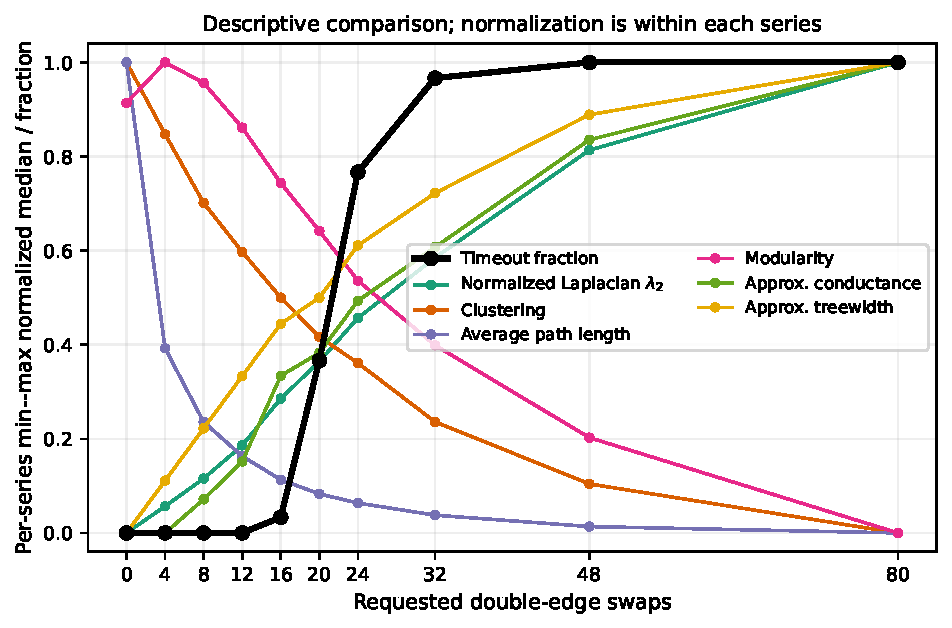
\includegraphics[width=.86\linewidth]{figures_20261003/normalized_structure_and_timeout.pdf}
\caption{Timeout fraction and min--max normalized structural medians. Each structural series is normalized independently across the ten perturbation levels. The comparison is descriptive and does not imply causality.}
\label{fig:normalized}
\end{figure}

\begin{table}[t]
\centering
\scriptsize
\caption{Median structural metrics by perturbation level. Conductance and treewidth are approximations.}
\label{tab:structure}
\begin{tabular}{rrrrrrrr}
\toprule
swaps & $p$ & $\lambda_2$ & clustering & avg. path & modularity & approx. conductance & approx. treewidth\\
\midrule
0  & .0000 & .0077 & .5000 & 10.380 & .6716 & .0714 & 4\\
4  & .0025 & .0163 & .4313 & 6.137  & .6908 & .0714 & 6\\
8  & .0050 & .0252 & .3656 & 5.044  & .6811 & .0882 & 8\\
12 & .0075 & .0359 & .3188 & 4.536  & .6598 & .1071 & 10\\
16 & .0100 & .0510 & .2750 & 4.186  & .6336 & .1500 & 12\\
20 & .0125 & .0630 & .2375 & 3.976  & .6109 & .1615 & 13\\
24 & .0150 & .0770 & .2125 & 3.840  & .5873 & .1875 & 15\\
32 & .0200 & .0965 & .1563 & 3.660  & .5567 & .2143 & 17\\
48 & .0300 & .1311 & .0969 & 3.491  & .5130 & .2679 & 20\\
80 & .0500 & .1594 & .0500 & 3.396  & .4678 & .3066 & 22\\
\bottomrule
\end{tabular}
\end{table}

The spectral gap is therefore a meaningful descriptor of increasing global connectivity, but it is not singled out as the explanation of censoring in this setting. The mixed outcomes at fixed perturbation levels also show that nearby $\lambda_2$ values can accompany very different solver outcomes.

\subsection{CDCL diagnostics across the transition}

Figure~\ref{fig:solver} summarizes three solver-side quantities. Median conflicts rise from approximately $4.0\times10^3$ at zero swaps to $4.4\times10^5$ at 16, $3.2\times10^6$ at 20, and more than $7.6\times10^6$ from 24 swaps onward. The solver does not simply become inactive. At the same time, median approximate mean LBD rises from 3.61 at zero swaps to 7.51, 8.97, and 11.44 at 16, 20, and 24 swaps, while median propagations per conflict falls from 9.35 to 3.99, 3.35, and 2.92.

\begin{figure}[t]
\centering
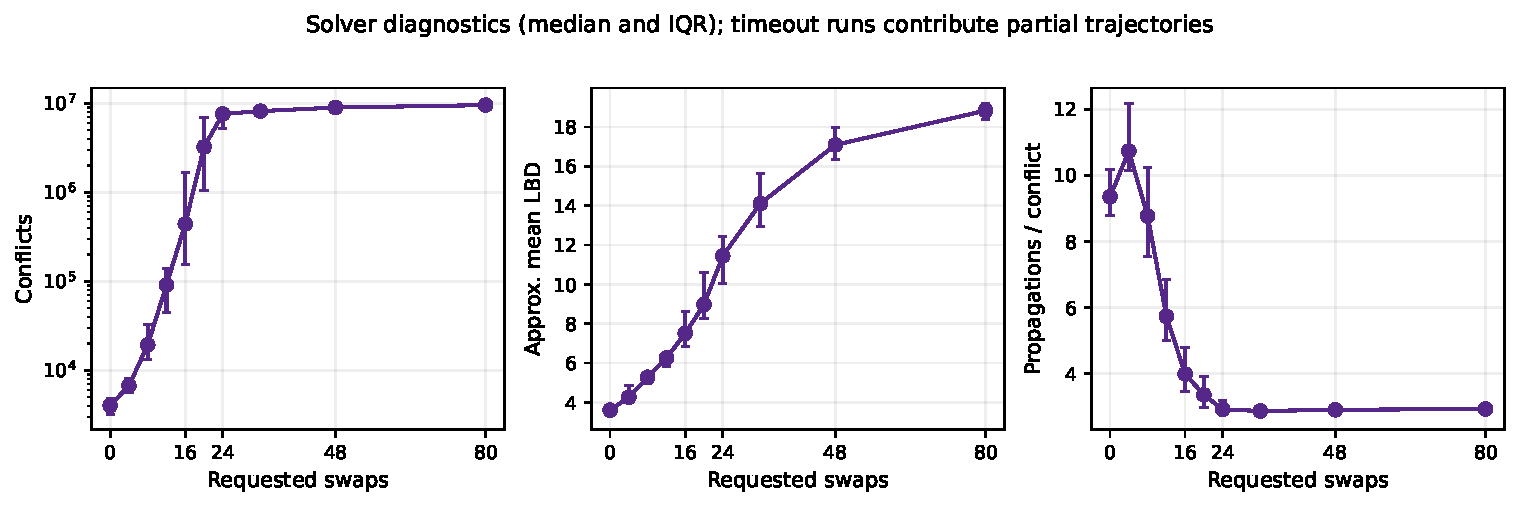
\includegraphics[width=\linewidth]{figures_20261003/solver_diagnostics_vs_requested_swaps.pdf}
\caption{Solver-trajectory diagnostics (median and IQR). Approximate mean LBD is the Kissat glue-bin proxy. Censored runs contribute measurements accumulated during their observed trajectories; their values are not completed-refutation statistics.}
\label{fig:solver}
\end{figure}

The transition is thus accompanied by sustained conflict activity, higher approximate LBD, and fewer propagations per conflict. These quantities can be causes, consequences, markers, or mutually coupled features of the increasingly censored regime. Because they aggregate over each observed trajectory, they do not establish temporal or causal direction.

Tracked-clause measurements provide a narrower complementary view (Figure~\ref{fig:tracked}). Median average usage remains of the same order across the campaign (6.85 at zero swaps and 6.58 at 80), and the median unused fraction remains small (0.016 and 0.009, respectively). Median lifetime rises from roughly $1.8\times10^3$ conflicts at zero swaps to more than $10^5$ at 48 and 80 swaps. The tracked database therefore remains active while run trajectories lengthen. These statistics apply only to large redundant learned clauses and should not be generalized to the entire clause database.

\begin{figure}[t]
\centering
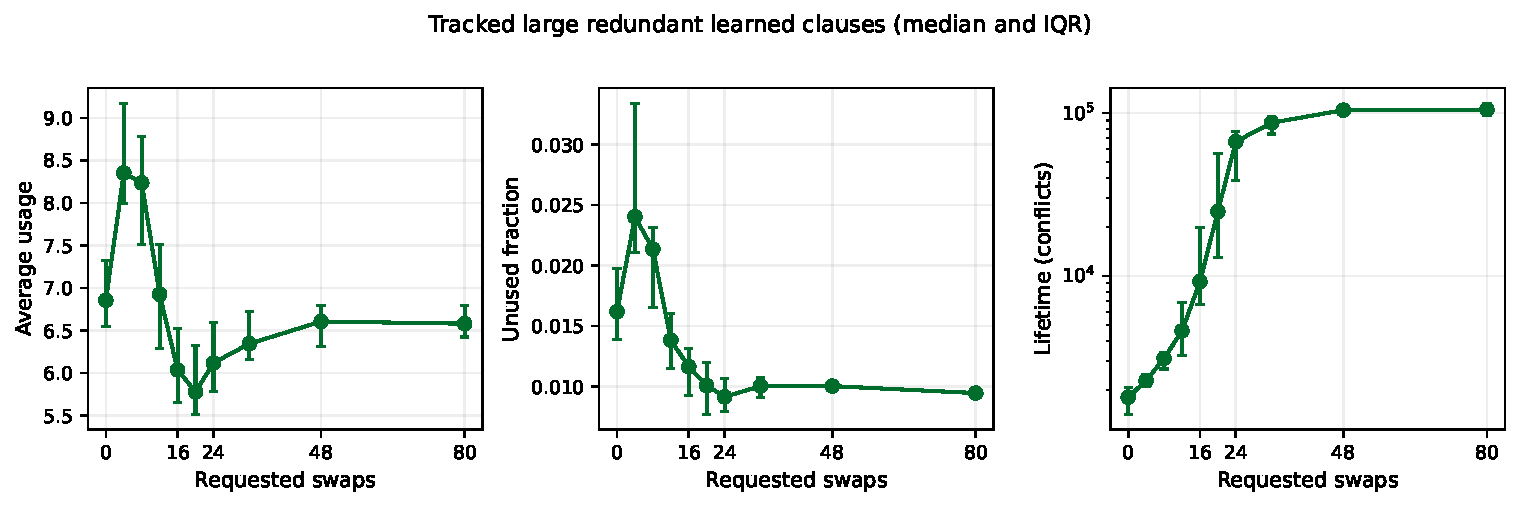
\includegraphics[width=\linewidth]{figures_20261003/tracked_clause_diagnostics_vs_requested_swaps.pdf}
\caption{Tracked large redundant learned-clause statistics (median and IQR). Usage counts propagation and conflict-analysis reuse; lifetime is measured in conflicts. Measurements are exact only within the tracked scope.}
\label{fig:tracked}
\end{figure}

\subsection{Within-level outcome variation}

Perturbation count alone does not determine the observed campaign outcome. At 20 requested swaps, 19 of 30 runs resolve and 11 are censored; at 24 swaps, 7 resolve and 23 are censored. Within either level, all graph--presentation pairs have identical $n$, $d$, $|E|$, degree sequence, and requested and successful swap counts, yet their budget statuses differ.

These observations document outcome heterogeneity at fixed perturbation count under the campaign presentations. They do not separate graph from presentation; the fixed-graph pilot (Section~\ref{sec:presentation}) and outcome-blind repeated-presentation campaign (Section~\ref{sec:robustness}) address that distinction directly.

\subsection{Independent confirmation at 20 and 24 swaps}

The confirmation campaign completed all 200 valid runs without execution errors: 111 resolved as \texttt{UNSAT} and 89 were right-censored as \texttt{UNKNOWN}, for an overall resolved fraction of 55.5\%. At 20 swaps, 75/100 (75\%) resolved; at 24 swaps, 36/100 (36\%) resolved. Table~\ref{tab:replication} reports the four prespecified fixed-stratum comparisons.

\begin{table}[H]
\centering
\scriptsize
\caption{Independent confirmation. Cliff's delta is censored minus resolved; CI denotes the deterministic 2,000-resample percentile-bootstrap interval. Holm adjustment applies only across the two modularity tests.}
\label{tab:replication}
\resizebox{\linewidth}{!}{%
\begin{tabular}{llrrrlll}
\toprule
metric & swaps & UNSAT & cens. & $\delta$ & 95\% CI & raw $p$ & Holm $p$\\
\midrule
global efficiency & 20 & 75 & 25 & $+0.626$ & $[0.429,0.791]$ & $3.09\times10^{-6}$ & --\\
global efficiency & 24 & 36 & 64 & $+0.621$ & $[0.444,0.774]$ & $2.88\times10^{-7}$ & --\\
modularity & 20 & 75 & 25 & $-0.663$ & $[-0.857,-0.457]$ & $7.66\times10^{-7}$ & $1.53\times10^{-6}$\\
modularity & 24 & 36 & 64 & $-0.589$ & $[-0.768,-0.386]$ & $1.14\times10^{-6}$ & $1.53\times10^{-6}$\\
\bottomrule
\end{tabular}
}
\end{table}

The primary hypothesis was confirmed under the frozen protocol: censored runs had higher global efficiency at both swap levels, with positive delta and raw $p<.05$ in each stratum. The secondary hypothesis was likewise confirmed: censored runs had lower modularity at both levels, with negative delta and Holm-adjusted $p<.05$ in each stratum. These decisions use only the independent sample. Each graph contributes one status under one frozen presentation, however, so these labels can be noisy measurements of a graph's propensity to exceed the budget across valid presentations.

The absolute effects are smaller than in the discovery data but retain their prespecified directions. For global efficiency, discovery deltas of $+0.88$ and $+0.84$ at 20 and 24 swaps became $+0.626$ and $+0.621$ in confirmation. For modularity, discovery deltas of $-0.81$ and $-0.73$ became $-0.663$ and $-0.589$. Timeout fractions also varied between samples: they were $11/30=0.367$ and $23/30=0.767$ in discovery, versus $25/100=0.250$ and $64/100=0.640$ in confirmation. Thus the replicated result is the direction-consistent within-swap association, not equality of timeout rates or effect magnitudes.

\subsection{Exploratory censored AFT analysis}
\label{sec:aft}

We fitted censored AFT models to the 60 discovery observations at 20 and 24 swaps (26 resolved, 34 censored). The main lognormal baseline contained a 24-versus-20-swap indicator and NetworkX min-fill treewidth; global efficiency and modularity were added separately. Continuous predictors were standardized from training data. Five-fold cross-validation grouped the two swap-level observations from each discovery seed in one fold, with zero seed overlap. Coefficients and discovery standardization were then applied to all 200 replication instances without refitting or restandardization.

Table~\ref{tab:aft} reports total changes in censored log likelihood and, in parentheses, changes per evaluated observation. The sample-size normalization matters because grouped cross-validation evaluates 60 observations and replication evaluates 200. Under the main lognormal model, efficiency gained $+5.036$ in cross-validation ($+0.084$ per observation) and $+26.748$ on replication ($+0.134$ per observation). Modularity gained $-0.077$ ($-0.001$ per observation) and $+25.421$ ($+0.127$ per observation), respectively.

In the main lognormal extensions, the coefficient for one discovery-sample standard deviation of global efficiency was $1.572$ on log time (95\% CI $[0.818,2.325]$), corresponding to a time ratio of $4.815$ (95\% CI $[2.266,10.230]$). The separately fitted modularity coefficient was $-1.297$ (95\% CI $[-2.030,-0.564]$), with time ratio $0.273$ (95\% CI $[0.131,0.569]$). These coefficients describe adjusted in-sample associations in separate models.

\begin{table}[H]
\centering
\scriptsize
\caption{Exploratory AFT log-likelihood gains over the stated baseline. Each score is total $\Delta\ell$ with mean $\Delta\ell$ per evaluated observation in parentheses. Replication uses the frozen discovery fit and standardization.}
\label{tab:aft}
\begin{tabular}{llrr}
\toprule
family; baseline & added metric & grouped CV: total (mean) & replication: total (mean)\\
\midrule
lognormal; swaps + min-fill treewidth & global efficiency & $+5.036$ ($+0.084$) & $+26.748$ ($+0.134$)\\
lognormal; swaps + min-fill treewidth & modularity & $-0.077$ ($-0.001$) & $+25.421$ ($+0.127$)\\
lognormal; baseline + $\lambda_2$ & global efficiency & $+3.580$ ($+0.060$) & $+17.480$ ($+0.087$)\\
lognormal; baseline + $\lambda_2$ & modularity & $-5.936$ ($-0.099$) & $+19.763$ ($+0.099$)\\
Weibull; swaps + min-fill treewidth & global efficiency & $+5.480$ ($+0.091$) & $+23.345$ ($+0.117$)\\
Weibull; swaps + min-fill treewidth & modularity & $+1.436$ ($+0.024$) & $+21.921$ ($+0.110$)\\
\bottomrule
\end{tabular}
\end{table}

We reconstructed the main-model replication contributions from the saved coefficients and frozen discovery standardization. A deterministic 20,000-resample bootstrap (seed 20261003), stratified by swap level and resampling graphs within the two 100-graph strata, gave a conditional 95\% percentile interval of $[+0.059,+0.211]$ for efficiency's mean paired gain and $[+0.041,+0.214]$ for modularity's. These intervals condition on the trained models and therefore exclude discovery-training uncertainty. No CV interval was computed because the original artifacts do not retain per-fold coefficients or per-observation predictions; recreating those quantities would require refitting the fold models.

The replication gains for efficiency and modularity are close, and no comparison of their superiority was tested. Across the evaluations performed, efficiency improved the score in the main CV, replication, the $\lambda_2$ sensitivity, and the Weibull sensitivity. Modularity improved replication and the Weibull CV but was approximately neutral in the main CV and negative in the $\lambda_2$ CV. Thus efficiency has the more consistent exploratory pattern across these checks, while modularity varies by evaluation. The two correlated metrics were fitted only as separate extensions, so their independent incremental contributions remain unassessed.

The baseline is approximate. Min-fill supplies a heuristic upper bound on treewidth and varies over a limited range within the two swap strata. The number of final edges differing from the seed-matched ring also varies at fixed requested swaps but was not included; it could account for part of the signal attributed to either structural metric. Exact treewidth was not computed.

\subsection{Exploratory fixed-graph presentation pilot}
\label{sec:presentation}

Eight replication graphs were selected after their earlier outcomes were known: within each of the 20- and 24-swap levels and each historical status, the first two rows by frozen plan index were chosen. Thus selection was deterministic but outcome-conditioned. Each graph had one byte-identical reference, three new odd-parity charges, three bijections of all 400 variable identifiers, and three permutations of all 1,040 clause positions. The 80 runs comprised 8 references and 24 variants in each family.

There were 53 \texttt{UNSAT}, 27 censored runs, and no error. Charges produced six \texttt{UNKNOWN}$\to$\texttt{UNSAT} changes. Variable numbering produced five \texttt{UNKNOWN}$\to$\texttt{UNSAT} and one \texttt{UNSAT}$\to$\texttt{UNKNOWN}; clause order produced four and one, respectively. Across families, 15 of the 36 variants derived from \texttt{UNKNOWN} references changed to \texttt{UNSAT}, whereas 2 of the 36 variants derived from \texttt{UNSAT} references changed to \texttt{UNKNOWN}. Because graph selection was conditioned on the original statuses, selection and regression toward the mean can contribute to this asymmetry. These proportions are descriptive for the eight selected graphs, not population rates.

All eight byte-identical reference reruns reproduced their historical status. This checks regeneration and status reproducibility for those eight reruns; it does not establish robustness across presentations. Table~\ref{tab:presentation} reports graph-level family counts. Variants are repeated runs on eight graphs, not independent graph samples. Resolved-only times and their denominators remain in the pilot artifacts; we do not compare them as an unconditional performance measure because censoring selects the resolved subset.

\begin{table}[H]
\centering
\scriptsize
\caption{Presentation pilot by fixed graph. Entries are \texttt{UNSAT}/censored counts; the reference column contains one byte-identical rerun per graph.}
\label{tab:presentation}
\begin{tabular}{rrlcccc}
\toprule
swaps & seed & historical & reference & charges & variables & clauses\\
\midrule
20 & 1000 & UNSAT   & 1/0 & 3/0 & 3/0 & 3/0\\
20 & 1001 & UNSAT   & 1/0 & 3/0 & 3/0 & 3/0\\
20 & 1004 & UNKNOWN & 0/1 & 1/2 & 0/3 & 0/3\\
20 & 1010 & UNKNOWN & 0/1 & 3/0 & 2/1 & 2/1\\
24 & 2001 & UNSAT   & 1/0 & 3/0 & 2/1 & 2/1\\
24 & 2002 & UNSAT   & 1/0 & 3/0 & 3/0 & 3/0\\
24 & 2000 & UNKNOWN & 0/1 & 2/1 & 3/0 & 1/2\\
24 & 2003 & UNKNOWN & 0/1 & 0/3 & 0/3 & 1/2\\
\midrule
\multicolumn{4}{r}{family totals} & 18/6 & 16/8 & 15/9\\
\bottomrule
\end{tabular}
\end{table}

For a connected graph, any two charges of the same total parity differ by a vector in the image of the graph incidence map over $\mathbb{F}_2$ and are related by complementing suitable edge variables. The odd-charge variants are therefore isomorphic contradictions under literal complementation. Together with variable and clause permutations, the pilot probes presentation-dependent solver behavior rather than a different satisfiability problem. The observed status changes are compatible with heuristic sensitivity, but wall-clock variation under the unrecorded machine conditions can also affect runs near 60 seconds; the current data do not fully separate these sources.

Three variants per family do not characterize a graph-level distribution over presentations. The following prespecified campaign addresses repeated joint variable-numbering and clause-order presentations in an outcome-blind graph sample.

\subsection{Prespecified presentation-robustness results}
\label{sec:robustness}

All 300 runs were valid: 180 resolved and 120 were \texttt{UNKNOWN}. The resolved fractions were 118/150 (78.7\%) at 20 swaps and 62/150 (41.3\%) at 24 swaps. For comparison, the single-presentation confirmation resolved 111/200 (55.5\%) overall, with 75\% and 36\% at the two levels. The campaigns use different graph samples and presentation procedures, so these descriptive percentages are not a test of temporal drift.

At graph level, 13 graphs resolved in 0/5 presentations, 24 had mixed outcomes (1--4/5), and 23 resolved in 5/5. The corresponding counts were 2, 12, and 16 at 20 swaps and 11, 12, and 7 at 24 swaps. The 24 mixed-status graphs document sensitivity in this sample under the specified presentation distribution; five repetitions do not estimate an individual graph's change rate precisely.

In the extension model, the standardized adjusted global-efficiency coefficient was $-1.525$ with graph-bootstrap 95\% interval $[-2.446,-0.688]$: higher efficiency was associated with a lower probability of resolution before 60 seconds. The held-out binary-log-score gain over the baseline was $+0.02265$, with conditional 95\% interval $[-0.01130,+0.05959]$. Adding squared standardized min-fill treewidth left the efficiency coefficient negative at $-1.480$ ($[-2.363,-0.702]$). The main fit and all main bootstrap fits converged without separation. The quadratic bootstrap accepted 4,911/5,000 fits; the other 89 converged numerically but triggered the frozen separation/ill-conditioning diagnostic. None was rank deficient or lacked covariate variation, and failed draws were not replaced.

The coefficient and direction criteria were met, whereas the predictive interval included zero. The frozen verdict is therefore \emph{robustness not established}. The adjusted association is supported under repeated presentations, while incremental predictive value remains inconclusive; the latter does not imply absence of an association. The signs differ from the exploratory AFT coefficient because the responses differ: a positive AFT coefficient means longer resolution time, whereas a negative binomial coefficient means a lower probability of resolving before 60 seconds.

\subsection{Exploratory effective-dose sensitivity}
\label{sec:effective-dose}

We reconstructed each seed-matched relabeled ring with the exact graph implementation and verified that all 60 reconstructed final edge sets matched the archived sources. We defined $m_{\mathrm{changed}}=|E_{\mathrm{final}}\setminus E_{\mathrm{ring}}|$; equal edge counts imply the same number removed from the ring and symmetric-difference size $2m_{\mathrm{changed}}$. At 20 swaps, $m_{\mathrm{changed}}$ ranged from 32 to 38 (median 35); at 24 it ranged from 38 to 46 (median 41). Its within-level correlations with efficiency were 0.414 and 0.265, and with treewidth 0.408 and 0.014, respectively.

Adding $m_{\mathrm{changed}}$ to the baseline gave an efficiency coefficient of $-1.472$ ($[-2.407,-0.608]$) in the extension. Its held-out score gain was $+0.0286$ with conditional interval $[-0.0017,+0.0627]$. The extension design condition number was 7.86 and VIFs ranged from 2.48 to 4.44; all full-sample, bootstrap, and CV fits were stable. Thus adjustment for effective dose left the efficiency association and inconclusive predictive interval materially similar. This weakens, but does not refute, the objection that effective dose alone accounts for the association. The sensitivity is exploratory, associational, and does not change the prespecified verdict.

\section{Discussion}

\subsection{Established results and bounded inference}

In the studied setting, the experiments establish three empirical results. The frozen independent confirmation replicated the prespecified within-swap associations of higher efficiency and lower modularity with censoring at 20 and 24 swaps. In the outcome-blind repeated-presentation sample, 24 of 60 graphs had both resolved and censored runs across five joint variable-numbering and clause-order presentations. The adjusted model recovered the expected negative association between efficiency and resolution probability.

The additional out-of-sample log-score gain was $+0.02265$, with conditional 95\% interval $[-0.01130,+0.05959]$. Because the interval included zero, the prespecified predictive criterion was not met and the frozen verdict remains \emph{robustness not established}. This supports the adjusted association across sampled presentations while leaving incremental predictive value inconclusive; it is not evidence of no effect.

The exploratory AFT and repeated-presentation analyses answer related but different questions. The former models censored solving time in 60 discovery graph--presentation pairs and evaluates frozen fits on the 200-instance confirmation. The latter models five binary budget outcomes per graph in a different, outcome-blind 60-graph sample. Its inconclusive predictive criterion limits generalization of the AFT pattern to repeated presentations; it does not directly contradict the positive AFT time coefficient. The effective-dose sensitivity left the repeated-presentation efficiency coefficient similar after adjustment for final changed edges, weakening but not eliminating that alternative explanation.

The solver trajectories also change systematically: conflict counts and approximate mean LBD rise, propagations per conflict fall, and tracked-clause lifetimes increase. These are trajectory-level associations accompanying the budget-crossing pattern, not a resolved causal mechanism.

These experiments measure observed search cost. No proof certificate was recorded, so they do not measure minimum proof size. The existence of polynomial-size refutations in stronger systems does not establish that Kissat's operations and heuristics efficiently realize those constructions.

\subsection{Limitations}

The experiments use $n=80$, $d=4$, one perturbation family, one Tseitin encoding, instrumented Kissat~4.0.4, and a 60-second wall-clock budget. The robustness result is specific to the joint distribution of uniform variable renumberings and clause permutations studied here; charges and within-clause literal order were fixed. The min-fill baseline is an upper bound on $\operatorname{tw}(G)$ computed on the original graph, not a direct estimate of $\operatorname{tw}(H)$ for the encoding gadget; $\operatorname{tw}(G)\leq\operatorname{tw}(H)$ does not turn that upper bound into a lower bound on proof difficulty. Exact treewidth was not computed. Efficiency, treewidth, and effective dose remain correlated, so the exploratory adjustment does not identify independent causal contributions.

With 60 graphs, the predictive contrast is estimated with limited precision. Its log-score-gain interval conditions on frozen out-of-fold predictions and omits full retraining variability; the coefficient bootstrap, by contrast, refits graph samples. The 89 unstable quadratic-bootstrap draws have no stable finite coefficient under the frozen estimator, so the consequence of their exclusion for an all-draw percentile interval cannot be evaluated. Wall-clock variation also remains inseparable from presentation-driven heuristic sensitivity for runs near the threshold.

\section{Conclusion}

Degree-preserving perturbation of the ring is associated with a rapid rise in 60-second censoring while graph size and degree sequence remain fixed. Independent confirmation reproduced the structural associations of higher global efficiency and lower modularity with censoring under the original protocol. In the repeated-presentation sample, 24 of 60 graphs had both resolved and censored outcomes, and the adjusted model recovered the association between higher efficiency and lower resolution probability.

The prespecified predictive requirement was not met: the efficiency extension's held-out log-score gain was $+0.02265$, with conditional 95\% interval $[-0.01130,+0.05959]$. Accordingly, robustness was not established, without implying absence of the adjusted association. The exploratory effective-dose adjustment produced a similar efficiency coefficient and the same inconclusive predictive pattern. Together, these results distinguish replicated structural association, presentation sensitivity, and incremental predictive evidence rather than treating them as one claim.

\appendix
\section{Canonical gadget representation}
\label{app:gadget}

To clarify the applicability of the cited proof-complexity results, for each original vertex $v$, the chained encoding replaces $v$ by a path of four vertices in $H$: three degree-three vertices corresponding to the successive XOR gates and one leaf. The three gate vertices have charge zero, while the leaf carries the original charge $q(v)$ and its canonical degree-one constraint is the unit clause in the campaign CNF. With the original incident edges attached to the gate path in the encoder's order, the canonical clauses of $T(H,q')$ coincide exactly with the three chained-XOR blocks and the unit clause, up to clause and literal order. Contracting each four-vertex gadget recovers $G$, so $G$ is a minor of $H$ and $\operatorname{tw}(G)\leq\operatorname{tw}(H)$. The reported min-fill value is only an upper bound on $\operatorname{tw}(G)$; it neither proves large treewidth nor instantiates a treewidth lower-bound premise.

\begin{thebibliography}{99}

\bibitem{Tseitin1970}
G.~S. Tseitin.
\newblock On the complexity of derivation in propositional calculus.
\newblock In \emph{Studies in Constructive Mathematics and Mathematical Logic, Part II}, pages 115--125. Consultants Bureau, 1970.

\bibitem{BenSassonWigderson2001}
Eli Ben-Sasson and Avi Wigderson.
\newblock Short proofs are narrow---Resolution made simple.
\newblock \emph{Journal of the ACM}, 48(2):149--169, 2001.
\newblock doi:10.1145/375827.375835.

\bibitem{AlekhnovichRazborov2011}
Michael Alekhnovich and Alexander~A. Razborov.
\newblock Satisfiability, branch-width and Tseitin tautologies.
\newblock \emph{Computational Complexity}, 20(4):649--678, 2011.
\newblock doi:10.1007/s00037-011-0033-1.

\bibitem{ItsyksonEtAl2022}
Dmitry Itsykson, Artur Riazanov, and Petr Smirnov.
\newblock Tight bounds for Tseitin formulas.
\newblock In \emph{SAT 2022}, LIPIcs 236, pages 6:1--6:21, 2022.
\newblock doi:10.4230/LIPIcs.SAT.2022.6.

\bibitem{deColnetMengel2023}
Alexis de Colnet and Stefan Mengel.
\newblock Characterizing Tseitin-formulas with short regular Resolution refutations.
\newblock \emph{Journal of Artificial Intelligence Research}, 76:265--286, 2023.
\newblock doi:10.1613/jair.1.13521.

\bibitem{BussThapen2021}
Sam Buss and Neil Thapen.
\newblock DRAT and propagation redundancy proofs without new variables.
\newblock \emph{Logical Methods in Computer Science}, 17(2):12:1--12:31, 2021.
\newblock doi:10.23638/LMCS-17(2:12)2021.

\bibitem{ChewHeule2020}
Leroy Chew and Marijn J.~H. Heule.
\newblock Sorting parity encodings by reusing variables.
\newblock In \emph{SAT 2020}, LNCS 12178, pages 1--10, 2020.
\newblock doi:10.1007/978-3-030-51825-7\_1.

\bibitem{ChewEtAl2024}
Leroy Chew, Alexis de Colnet, Friedrich Slivovsky, and Stefan Szeider.
\newblock Hardness of random reordered encodings of parity for Resolution and CDCL.
\newblock In \emph{AAAI 2024}, pages 7978--7986, 2024.
\newblock doi:10.1609/aaai.v38i8.28635.

\bibitem{GomesEtAl1998}
Carla~P. Gomes, Bart Selman, and Henry~A. Kautz.
\newblock Boosting combinatorial search through randomization.
\newblock In \emph{AAAI 1998}, pages 431--437, 1998.

\bibitem{GomesEtAl2000}
Carla~P. Gomes, Bart Selman, Nuno Crato, and Henry~A. Kautz.
\newblock Heavy-tailed phenomena in satisfiability and constraint satisfaction problems.
\newblock \emph{Journal of Automated Reasoning}, 24(1--2):67--100, 2000.
\newblock doi:10.1023/A:1006314320276.

\bibitem{GomesSabharwal2021}
Carla~P. Gomes and Ashish Sabharwal.
\newblock Exploiting runtime variation in complete solvers.
\newblock In Armin Biere, Marijn Heule, Hans van Maaren, and Toby Walsh, editors,
\emph{Handbook of Satisfiability}, second edition, pages 463--480.
IOS Press, 2021.
\newblock doi:10.3233/FAIA200994.

\bibitem{WattsStrogatz1998}
Duncan~J. Watts and Steven~H. Strogatz.
\newblock Collective dynamics of small-world networks.
\newblock \emph{Nature}, 393:440--442, 1998.
\newblock doi:10.1038/30918.

\bibitem{Roli2005}
Andrea Roli.
\newblock On the impact of small-world on local search.
\newblock In \emph{AI*IA 2005: Advances in Artificial Intelligence}, LNCS 3673, pages 13--24, 2005.
\newblock doi:10.1007/11558590\_2.

\bibitem{AnsoteguiEtAl2012}
Carlos Ansótegui, Jesús Giráldez-Cru, and Jordi Levy.
\newblock The community structure of SAT formulas.
\newblock In \emph{SAT 2012}, LNCS 7317, pages 410--423, 2012.
\newblock doi:10.1007/978-3-642-31612-8\_31.

\bibitem{AnsoteguiEtAl2015}
Carlos Ansótegui, Jesús Giráldez-Cru, Jordi Levy, and Laurent Simon.
\newblock Using community structure to detect relevant learnt clauses.
\newblock In \emph{SAT 2015}, LNCS 9340, pages 238--254, 2015.
\newblock doi:10.1007/978-3-319-24318-4\_18.

\bibitem{AnsoteguiEtAl2019}
Carlos Ansótegui, Maria~Luisa Bonet, Jesús Giráldez-Cru, Jordi Levy, and Laurent Simon.
\newblock Community structure in industrial SAT instances.
\newblock \emph{Journal of Artificial Intelligence Research}, 66:443--472, 2019.
\newblock doi:10.1613/JAIR.1.11741.

\bibitem{ElffersEtAl2018}
Jan Elffers, Jesús Giráldez-Cru, Stephan Gocht, Jakob Nordström, and Laurent Simon.
\newblock Seeking practical CDCL insights from theoretical SAT benchmarks.
\newblock In \emph{IJCAI 2018}, pages 1300--1308, 2018.
\newblock doi:10.24963/ijcai.2018/181.

\bibitem{AudemardSimon2009}
Gilles Audemard and Laurent Simon.
\newblock Predicting learnt clauses quality in modern SAT solvers.
\newblock In \emph{IJCAI 2009}, pages 399--404, 2009.
\newblock doi:10.5555/1661445.1661509.

\bibitem{BussEtAl2026}
Sam Buss, Jonathan Chung, Vijay Ganesh, and Albert Oliveras.
\newblock Extended Resolution Clause Learning via dual implication points.
\newblock \emph{Logical Methods in Computer Science}, 22(2):23, 2026.
\newblock doi:10.46298/lmcs-22(2:23)2026.

\bibitem{BeameSun2026}
Paul Beame and Glenn Sun.
\newblock Extending CDCL to disjunctions of parity equations.
\newblock In Alexey Ignatiev and Stefan Szeider, editors, \emph{SAT 2026}, LIPIcs 377, pages 5:1--5:21, 2026.
\newblock doi:10.4230/LIPIcs.SAT.2026.5.

\bibitem{ZhangEtAl2026}
Shimin Zhang, Yechuan Xia, Chunxiao Li, Jianwen Li, Moshe~Y. Vardi, and Vijay Ganesh.
\newblock Understanding CDCL solvers via scalability studies and proofdoors.
\newblock In Bruno Dutertre and Bettina Könighofer, editors, \emph{Proceedings of the 26th Conference on Formal Methods in Computer-Aided Design (FMCAD 2026)}, pages 37--49. TU Wien Academic Press, 2026.
\newblock doi:10.34727/2026/isbn.978-3-85448-093-8\_9.

\bibitem{SinghEtAl2026}
Sunidhi Singh, Vincent Liew, Marc Vinyals, and Vijay Ganesh.
\newblock Proofdoors and efficiency of CDCL solvers.
\newblock arXiv:2603.26286, 2026.

\end{thebibliography}

\end{document}
